\section{Suitable evaluation test}

%Anledningen till att vi vill göra detta test är att se om det är möjligt att använda sig av ICNs pull strategi för att hämta data kontinuerligt från en sensor. Det vore intressant att se om det är möjligt att skapa ett system där användaren får datat så fort det har skapats hos sensorn, där tiden det tar från att datat har skapats tills dess att användaren har det är så liten som möjligt. Vanligtvis användes diverse publish subscribe system som t.ex MQTT för att erhålla datat så snabbt som möjligt som användare. Där pushas datat ut från sensorn då det tillverkats. Istället för denna push model, är det av intresse att utvärdera ICNs pull strategi tillsammans med `one-time subscription'-modellen som Ahlgren et al beskriver i [ref.]. Resultatet visar om det är möjligt att combinera de två tänken för att erhålla datat så snabbt som möjligt samt hur stabilt ett sådant system skulle kunna tänkas vara.  

%The result show if such a possibility exists with data produced with a constant interval over a long period of time. 
%The communication patterns of ICN and CCN is by natural pull-based, which is in contradiction to a regular publish/subscribe protocol such as MQTT. When using a publish/subscribe communication protocol, it can send the newly produced data directly towards a consumer. 

%With the CCN possibility of storing \textit{interest} requests at the sensors, combined with the `one-time' subscription approach described by Ahlgrens et al[ref], it could be possible to achive the same functionallity with ICN. It is interesting to see how such a combination would perform over time. 

%%
%The reason to do this experiement is to see if it is possible to use the ICNs pull strategy to retrieve data continuously from a sensor. 

%\begin{itemize}
%\item retreieve data ass soon as it has been possible.
%\item one time subscription
%\item long time interval
%\item Follow sequence and periodicity from sensor
%\item The interval time between the data created by the sensor is known beforehand from the requestor.
%\item refer to MQTT difference
%\item CCN.
%\end{itemize}
The purpose of this experiment is to create a suitable software for a consumer toat follows an interval and retrieves the data which is created periodically by a sensor node. A key goal is enabling the consumer to recieve the data as soon as it has been created at the sensor. The interval when the data is created could be of arbitray, but fixed, length.  Usually, a publish subscribe communication such as MQTT handles this by pushing the data towards the consumer as soon as it is created. 
With the CCN possibility of storing \textit{interest} requests at the sensors combined with the `one-time' subscription approach, described by Ahlgrens et al in \cite{Ahlgreniot} where the consumer sends an \textit{interest} in advance for future data, it could be possible to achive the same functionallity with ICN. The results show how such an system would perform over time and if it is a feasible replacement to the publish subscribe approach. 

Although the purpose is to follow the sequence numbering of the data, it is out of the scope of this thesis to find the latest sequence number. This is considered to be known for the system in advance.
%\subsection{Delim}
%It is not a purpose to find the latest sequence number, this is given at first hand. There are several different types of techniques to get the latest sequence number, but it is out of scope of this paper. 
\subsection{Method}
%%\begin{itemize}
%%\item Follow interval on sensor, becomes a problem due to the fact that there is two different clocks. One on sensor that is producing at a certain interval speed, and one %%at the client that wants to consume at a regular interval speed.
%%\item Come to the right sensor
%%\item First timeout, usage of PIT, one time subscription model. Describe the one time subscription model.
%%\item After timeout, Algoritm usage to follow/correct
%%\item The algoritm.\\
%%\end{itemize}

%\begin{itemize}
%\item Algorithm
%\end{itemize}
The algorithm developed in this project, shown in figure \ref{fig:onetime}, is a first attempt to retreive data with the previously described one time subscription approach. 
The algorithm tries to fetch data at a certain interval in order to recieve the data as soon as it has been created on the sensor. It calculates when to send the next request towards the sensor, based on the round trip time of the current interval. The smoothed round trip time (srtt) technique makes the system more tolerant when handeling a latency value differs substantially from usual. One must set a round trip target (rtt$\_$target) that the algortihm follows. It is a factor of the minimum round trip time (rtt$\_$min). In the algortihm, there is a background correction factor that is calculated at every interval. This correction time is the difference between the srtt and the rtt$\_$target. It represents the difference in time between the two systems. Together with the interval rate at which the data is produced and when the current interval started, the correction factor is added in order to decide when to send the next request. \\\\
%\begin{itemize}
%\item diff rttmin rtt$\_$target
%\end{itemize}
The reason for using the rtt$\_$target is the need to send the \textit{interest} request at a comfortable distance before the data has been created.
When using the pit of CCN, one can not retrieve the same latency values as in the previous measurement where the data was replied directly from the sensors cache. Instead, one must set a round trip target that is related to the rtt$\_$min. The difference between rtt$\_$target and rtt$\_$min defines how long the time span which the algorithm can regulate is. The smaller the differences, the more vulnerable the system becomes for variations of rtt. The minimum difference must be greater than the differences of the two intervals between the sensor and the gateway. If it gets less, the algortihm stops working properly.\\\\
%\begin{itemize}
%\item Smoothed RTT
%\end{itemize}
In order to calculate when to send the next request towards the sensor, one could subtract the rtt from the interval. 
However, this makes the system more sensitive to changes in the latencies which could lead to timeouts for a consumer. To solve this issue and make the latencies more stable over time, a smoothed rtt is used in the algortihm. It uses a factor $\alpha$, to decide how the current round trip time should be weighted in comparison to the previous latency values. The greater $\alpha$ becomes, the less importance the older values have. When $\alpha$ becomes smaller, the weighting of older values grows.
If the latencies of the srtt is high, the \textit{interest} request is sent too early towards the sensor. At the same time, if the srtt latency becomes to short, the request is sent to late.\\\\
%%\begin{itemize}
%%\item Corr \\
%%	The difference in clock time between the sensor and the gw is measured with corr.
%%\end{itemize}

   
\begin{figure}
\begin{algorithm}[H]
 next = reference time\;
 rtt$\_$min\;
 rtt$\_$target = rtt$\_$min * \textit{x}\;
 $\alpha$ = 0 <= $\alpha$ <= 1\;
 \While{infinity}{
  rtt = send$\_$interest$\_$receive$\_$data\;
  \If{not timeout}{
   srtt = $\alpha$ $\times$ rtt + ($\alpha$ - 1) $\times$  srtt\;
   corr = srtt - rtt$\_$target\;
   }
   next$\_$time = next$\_$time + interval$\_$time + corr\;
   sleep(next$\_$time - current$\_$time)\;
 }

\end{algorithm}
\caption{Algorithm that makes it possible for a consumer to follow the creation of data with a certain interval.}
    \label{fig:onetime}
\end{figure}


\subsection{Result}
%\begin{itemize}
%\item Show that the algorithm can follow the interval and period over time. (show this with standard case 0.1 first.)\\
%\end{itemize}
The results regarding latencies when using $\alpha$ = 0.1 and \textit{rtt$\_$target} = 2.5 is shown in figure \ref{fig:gw/test/alpha/0.1/rtttarget/2.5/diff/1.0/slope/0.15/zommed}. The interval sequence number is plotted on the x-axis and the roundtrip latency is plotted on the y-axis. The same axis layout holds for all figures of which regard the round trip times from the gateway/consumers perspective. 
The results, illustrated in figure \ref{fig:gw/test/alpha/0.1/rtttarget/2.5/diff/1.0/slope/0.15/zommed}, shows that the latency is stable between 90-100 ms, the srtt is stable with a small variance around 95 ms and that the correlation is stable around 5 ms as well. This results indicate that the consumer can retrieve the data in a stable manner.\\\\
The corresponding time from a sensors perspective is shown in figure \ref{fig:sensor/test/alpha/0.1/rtttarget/2.5/diff/1.0/slope/0.15/zommed}, where the interval sequence number is plotted on the x-axis and the age of the data is plotted on the y-axis. When the values become negative, the sensor makes use of the CCN pit. They show the time between recieving the \textit{interest} until the \textit{data} was created and responded towards the requestor. The same axis format holds for all figures regarding the age of the data at the sensor. Figure \ref{fig:sensor/test/alpha/0.1/rtttarget/2.5/diff/1.0/slope/0.15/zommed}, which corresponds to when $\alpha$ = 0.1 and \textit{rtt$\_$target} = 2.5, shows that the age of the \textit{interest} is very stable at 62 ms (8 tick). \\Small variances in the age of the interest indicates that the algorithm to request the values is stable and that the use of the pit is working properly.\\\\
%\begin{itemize}
%\item Show difference between using $\alpha$ = 0.1, 0.9 and 1.
%\end{itemize}
When $\alpha$ is changed to 0.9, the resulting curves, illustrated in figure \ref{fig:gw/test/alpha/0.9/rtttarget/2.5/diff/1.0/slope/0.15/zommed} and \ref{fig:sensor/test/alpha/0.9/rtttarget/2.5/diff/1.0/slope/0.15/zommed}, show more alternating forms. The latencies range from 87 ms to 117 ms, and most ofthen they are either at the both ends spectrum or at 97 ms. The age of the \textit{interests} is at the same time pending between 56 ms to 70 ms. This is due to the fact that the srtt has less importance and influence as $\alpha$ grows. Instead, the time when next interest is sent is more depending on the current latency time. 
These results show that the algorithm has no problem handling a shifting rtt and that the system stays stable. When the rtts start to alternate, it is hard for the system to stop.\\\\
When $\alpha$ is set to 1, illustrated in figure \ref{fig:gw/test/alpha/1.0/rtttarget/2.5/diff/1.0/slope/0.15/zommed} and \ref{fig:sensor/test/alpha/1.0/rtttarget/2.5/diff/1.0/slope/0.15/zommed}, the latency times alternate between 87 ms and 117 ms as seen with $\alpha$ = 0.9, but here the frequency is greater. In this case, the smoothing is not available and therefore the correction is only dependent on the last roundtrip time. The algorithm works and can easily handle when changing $\alpha$ to 0.9 or 1, but this is also due to the high rtt$\_$target.  If the gap between rtt$\_$target and rtt$\_$min shrinks, the risk of instability and retrieving older data grows.

\subsubsection{Different intervals at the sensor}
%\begin{itemize}
%\item Show that it can handle diff in the interval. The producer has a different interval than the consumer. Works great without problems for positive changes, where the %producer is creating the data at a slower interval, say 1.2 second per data.
%\item Show difference in time. 
%\end{itemize}
All of the previous results were made under the assumption that the two intervals are relatively the same. One interval second on the sensor is almost the same as one interval second on the GW. To illustrate the functionallity when the sensor is providing data at different periodicity than the GW, other tests have been made. The algorithm proves to stay stable even for variances in the drift time caused by the sensor. \\\\
In figure \ref{fig:gw/test/alpha/0.1/rtttarget/2.5/diff/1.02/slope/0.15/zommed} and \ref{fig:sensor/test/alpha/0.1/rtttarget/2.5/diff/1.02/slope/0.15/zommed}, the sensor is creating the data with an interval of one second + 2$\%$ and the gateway still uses an interval period of one second. The results show that the system is still stable over time, even though here is a positive drift in time on the sensor. The time it takes for an \textit{interest} to be consumed by the sensor is around 78 ms. The latency from the gw is overall higher, 105 ms to 125 ms, in comparission to without any difference in the time intervals, but the variation of srtt is still small and at the same levels. This is logic since the \textit{interest} is sent earlier from the gateway towards the sensor, but at the the same intervals, due to the algorithm. However, there is a cap, when the \textit{interests} start to timeout, the system will stop working properly and no data will be received at the gw. The drift on the sensor compared to the gateway cannot be greater than the timeout that the gw is setting on the \textit{interest}-packet when it is issued. Furthermore, the srtt is always greater than rtt$\_$target which provides stability in the system.\\\\
%\begin{itemize}
%	\item show diff in time negative, shorter time.
%\end{itemize}
Additionally, at a smaller sensor period of -2$\%$ compared to the gateway-interval, the system stays stable. The roundtrips as well as the age of the interests are smaller than when the two intervals are the same and the age of the \textit{interests} are smaller too. The majority of latencies is between 65 to 75 ms, as seen in figure \ref{fig:gw/test/alpha/0.1/rtttarget/2.5/diff/0.98/slope/0.15/zommed}, and the time it took to consume the interest was around 40 ms as seen in figure \ref{fig:sensor/test/alpha/0.1/rtttarget/2.5/diff/0.98/slope/0.15/zommed}. The reason why this is still stable is because the difference between rtt$\_$target and rtt$\_$min, 88 ms - 38 ms = 50 ms, is greater than the negative drift of -2 $\%$, approximatly 23 ms, of the sensors interval clock. Once the drift exceeds the difference between rtt$\_$min and rtt$\_$target, the algortihm is unstable and it stops working properly.




%%%%%%%%%%%%%%%% FIGURES!!! %%%%%%%%%%%%%%%%%%%
\begin{figure}\centering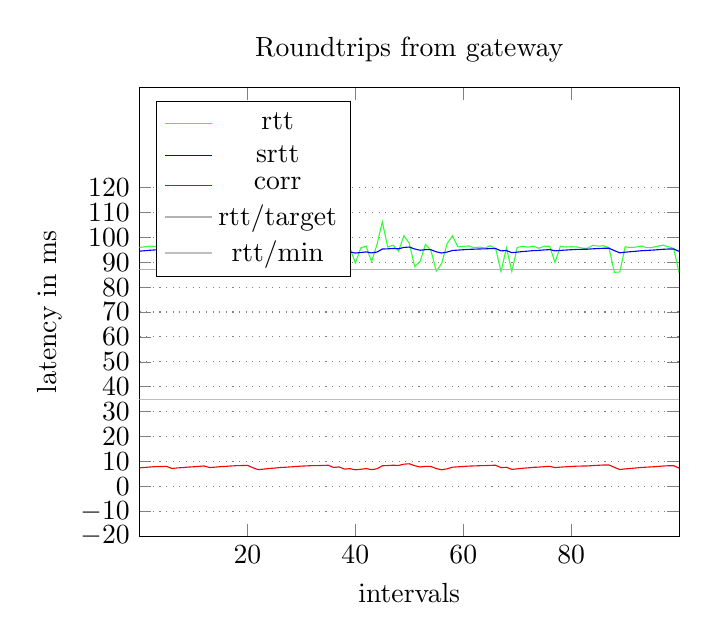
\begin{tikzpicture}\begin{axis}[
title={Roundtrips from gateway},
xlabel={intervals}, ylabel={latency in ms},
xmin=0, xmax=700,ymin=-20, ymax=160,
xtick={100,200,300,400,500,600},
xmin=000, xmax=100,ymin=-20, ymax=160,
xtick={20,40,60,80},
ytick={-40,-30,-20,-10,0,10,20,30,40,50,60,70,80,90,100,110,120},
legend pos=north west, grid style={dotted,gray},ymajorgrids=true,]
\addplot[ color=green!80 ] coordinates {(0,95.892)(1,96.225)(2,96.477)(3,96.295)(4,95.182)(5,95.829)(6,86.47)(7,96.382)(8,95.885)(9,96.507)(10,95.97)(11,96.58)(12,96.637)(13,88.907)(14,96.141)(15,96.673)(16,96.168)(17,96.645)(18,96.467)(19,95.839)(20,96.043)(21,86.094)(22,86.646)(23,95.839)(24,96.572)(25,95.793)(26,96.453)(27,95.827)(28,96.094)(29,96.458)(30,96.543)(31,96.148)(32,96.32)(33,95.226)(34,96.43)(35,95.8)(36,86.612)(37,96.915)(38,85.968)(39,95.738)(40,89.69)(41,95.701)(42,96.486)(43,90.232)(44,97.04)(45,106.198)(46,96.115)(47,96.835)(48,94.404)(49,100.659)(50,97.566)(51,88.262)(52,90.275)(53,97.162)(54,94.851)(55,86.398)(56,89.476)(57,97.457)(58,100.57)(59,96.148)(60,96.366)(61,96.524)(62,95.852)(63,96.07)(64,95.707)(65,96.569)(66,95.53)(67,86.282)(68,95.782)(69,86.324)(70,95.897)(71,96.418)(72,96.034)(73,96.452)(74,95.587)(75,96.438)(76,96.402)(77,89.975)(78,96.43)(79,96.109)(80,96.207)(81,96.143)(82,95.691)(83,95.529)(84,96.816)(85,96.447)(86,96.616)(87,95.805)(88,85.989)(89,86.005)(90,96.192)(91,95.902)(92,96.081)(93,96.495)(94,95.853)(95,95.884)(96,96.421)(97,96.83)(98,96.239)(99,95.535)(100,85.692)};\addlegendentry{rtt}
\addplot[ color=blue ] coordinates {(0,94.4488858585)(1,94.6264972726)(2,94.8115475454)(3,94.9598927908)(4,94.9821035117)(5,95.0667931606)(6,94.2071138445)(7,94.4246024601)(8,94.5706422141)(9,94.7642779927)(10,94.8848501934)(11,95.054365174)(12,95.2126286566)(13,94.582065791)(14,94.7379592119)(15,94.9314632907)(16,95.0551169616)(17,95.2141052655)(18,95.3393947389)(19,95.389355265)(20,95.4547197385)(21,94.5186477647)(22,93.7313829882)(23,93.9421446894)(24,94.2051302204)(25,94.3639171984)(26,94.5728254786)(27,94.6982429307)(28,94.8378186376)(29,94.9998367739)(30,95.1541530965)(31,95.2535377868)(32,95.3601840082)(33,95.3467656073)(34,95.4550890466)(35,95.4895801419)(36,94.6018221277)(37,94.833139915)(38,93.9466259235)(39,94.1257633311)(40,93.682186998)(41,93.8840682982)(42,94.1442614684)(43,93.7530353216)(44,94.0817317894)(45,95.2933586105)(46,95.3755227494)(47,95.5214704745)(48,95.409723427)(49,95.9346510843)(50,96.0977859759)(51,95.3142073783)(52,94.8102866405)(53,95.0454579764)(54,95.0260121788)(55,94.1632109609)(56,93.6944898648)(57,94.0707408783)(58,94.7206667905)(59,94.8634001114)(60,95.0136601003)(61,95.1646940903)(62,95.2334246812)(63,95.3170822131)(64,95.3560739918)(65,95.4773665926)(66,95.4826299334)(67,94.56256694)(68,94.684510246)(69,93.8484592214)(70,94.0533132993)(71,94.2897819694)(72,94.4642037724)(73,94.6629833952)(74,94.7553850557)(75,94.9236465501)(76,95.0714818951)(77,94.5618337056)(78,94.748650335)(79,94.8846853015)(80,95.0169167714)(81,95.1295250942)(82,95.1856725848)(83,95.2200053263)(84,95.3796047937)(85,95.4863443143)(86,95.5993098829)(87,95.6198788946)(88,94.6567910051)(89,93.7916119046)(90,94.0316507142)(91,94.2186856427)(92,94.4049170785)(93,94.6139253706)(94,94.7378328336)(95,94.8524495502)(96,95.0093045952)(97,95.1913741357)(98,95.2961367221)(99,95.3200230499)(100,94.3572207449)};\addlegendentry{srtt}
\addplot[ color=red ] coordinates {(0,7.43138585847)(1,7.60899727263)(2,7.79404754536)(3,7.94239279083)(4,7.96460351175)(5,8.04929316057)(6,7.18961384451)(7,7.40710246006)(8,7.55314221406)(9,7.74677799265)(10,7.86735019339)(11,8.03686517405)(12,8.19512865664)(13,7.56456579098)(14,7.72045921188)(15,7.91396329069)(16,8.03761696162)(17,8.19660526546)(18,8.32189473891)(19,8.37185526502)(20,8.43721973852)(21,7.50114776467)(22,6.7138829882)(23,6.92464468938)(24,7.18763022044)(25,7.3464171984)(26,7.55532547856)(27,7.6807429307)(28,7.82031863763)(29,7.98233677387)(30,8.13665309648)(31,8.23603778683)(32,8.34268400815)(33,8.32926560734)(34,8.4375890466)(35,8.47208014194)(36,7.58432212775)(37,7.81563991497)(38,6.92912592348)(39,7.10826333113)(40,6.66468699802)(41,6.86656829821)(42,7.12676146839)(43,6.73553532155)(44,7.0642317894)(45,8.27585861046)(46,8.35802274941)(47,8.50397047447)(48,8.39222342702)(49,8.91715108432)(50,9.08028597589)(51,8.2967073783)(52,7.79278664047)(53,8.02795797642)(54,8.00851217878)(55,7.1457109609)(56,6.67698986481)(57,7.05324087833)(58,7.7031667905)(59,7.84590011145)(60,7.9961601003)(61,8.14719409027)(62,8.21592468125)(63,8.29958221312)(64,8.33857399181)(65,8.45986659263)(66,8.46512993337)(67,7.54506694003)(68,7.66701024603)(69,6.83095922142)(70,7.03581329928)(71,7.27228196935)(72,7.44670377242)(73,7.64548339518)(74,7.73788505566)(75,7.90614655009)(76,8.05398189508)(77,7.54433370557)(78,7.73115033502)(79,7.86718530152)(80,7.99941677136)(81,8.11202509423)(82,8.1681725848)(83,8.20250532632)(84,8.36210479369)(85,8.46884431432)(86,8.58180988289)(87,8.6023788946)(88,7.63929100514)(89,6.77411190463)(90,7.01415071416)(91,7.20118564275)(92,7.38741707847)(93,7.59642537063)(94,7.72033283356)(95,7.83494955021)(96,7.99180459519)(97,8.17387413567)(98,8.2786367221)(99,8.30252304989)(100,7.3397207449)};\addlegendentry{corr}
\addplot[ color=gray!60 ] coordinates {(0,87.0175)(1,87.0175)(2,87.0175)(3,87.0175)(4,87.0175)(5,87.0175)(6,87.0175)(7,87.0175)(8,87.0175)(9,87.0175)(10,87.0175)(11,87.0175)(12,87.0175)(13,87.0175)(14,87.0175)(15,87.0175)(16,87.0175)(17,87.0175)(18,87.0175)(19,87.0175)(20,87.0175)(21,87.0175)(22,87.0175)(23,87.0175)(24,87.0175)(25,87.0175)(26,87.0175)(27,87.0175)(28,87.0175)(29,87.0175)(30,87.0175)(31,87.0175)(32,87.0175)(33,87.0175)(34,87.0175)(35,87.0175)(36,87.0175)(37,87.0175)(38,87.0175)(39,87.0175)(40,87.0175)(41,87.0175)(42,87.0175)(43,87.0175)(44,87.0175)(45,87.0175)(46,87.0175)(47,87.0175)(48,87.0175)(49,87.0175)(50,87.0175)(51,87.0175)(52,87.0175)(53,87.0175)(54,87.0175)(55,87.0175)(56,87.0175)(57,87.0175)(58,87.0175)(59,87.0175)(60,87.0175)(61,87.0175)(62,87.0175)(63,87.0175)(64,87.0175)(65,87.0175)(66,87.0175)(67,87.0175)(68,87.0175)(69,87.0175)(70,87.0175)(71,87.0175)(72,87.0175)(73,87.0175)(74,87.0175)(75,87.0175)(76,87.0175)(77,87.0175)(78,87.0175)(79,87.0175)(80,87.0175)(81,87.0175)(82,87.0175)(83,87.0175)(84,87.0175)(85,87.0175)(86,87.0175)(87,87.0175)(88,87.0175)(89,87.0175)(90,87.0175)(91,87.0175)(92,87.0175)(93,87.0175)(94,87.0175)(95,87.0175)(96,87.0175)(97,87.0175)(98,87.0175)(99,87.0175)(100,87.0175)};\addlegendentry{rtt/target}
\addplot[ color=gray!50  ] coordinates {(0,34.807)(1,34.807)(2,34.807)(3,34.807)(4,34.807)(5,34.807)(6,34.807)(7,34.807)(8,34.807)(9,34.807)(10,34.807)(11,34.807)(12,34.807)(13,34.807)(14,34.807)(15,34.807)(16,34.807)(17,34.807)(18,34.807)(19,34.807)(20,34.807)(21,34.807)(22,34.807)(23,34.807)(24,34.807)(25,34.807)(26,34.807)(27,34.807)(28,34.807)(29,34.807)(30,34.807)(31,34.807)(32,34.807)(33,34.807)(34,34.807)(35,34.807)(36,34.807)(37,34.807)(38,34.807)(39,34.807)(40,34.807)(41,34.807)(42,34.807)(43,34.807)(44,34.807)(45,34.807)(46,34.807)(47,34.807)(48,34.807)(49,34.807)(50,34.807)(51,34.807)(52,34.807)(53,34.807)(54,34.807)(55,34.807)(56,34.807)(57,34.807)(58,34.807)(59,34.807)(60,34.807)(61,34.807)(62,34.807)(63,34.807)(64,34.807)(65,34.807)(66,34.807)(67,34.807)(68,34.807)(69,34.807)(70,34.807)(71,34.807)(72,34.807)(73,34.807)(74,34.807)(75,34.807)(76,34.807)(77,34.807)(78,34.807)(79,34.807)(80,34.807)(81,34.807)(82,34.807)(83,34.807)(84,34.807)(85,34.807)(86,34.807)(87,34.807)(88,34.807)(89,34.807)(90,34.807)(91,34.807)(92,34.807)(93,34.807)(94,34.807)(95,34.807)(96,34.807)(97,34.807)(98,34.807)(99,34.807)(100,34.807)};\addlegendentry{rtt/min}
\end{axis}\end{tikzpicture}
\caption{gw/test/alpha/0.1/rtttarget/2.5/diff/1.0/slope/0.15/zommed}
\label{fig:gw/test/alpha/0.1/rtttarget/2.5/diff/1.0/slope/0.15/zommed}
\end{figure}

\begin{figure}\centering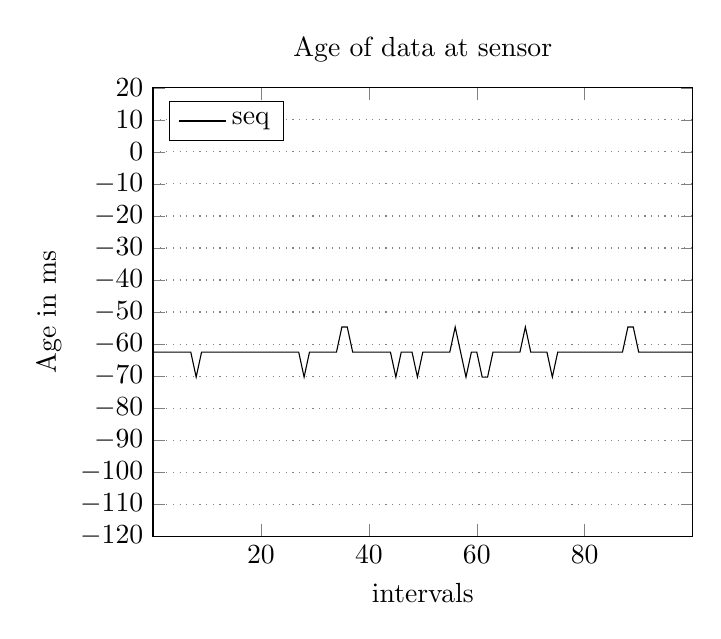
\begin{tikzpicture}\begin{axis}[
title={Age of data at sensor},
xlabel={intervals}, ylabel={Age in ms},
xmin=000, xmax=100,ymin=-120, ymax=20,
xtick={20,40,60,80},
ytick={-120,-110, -100,-90,-80,-70,-60,-50,-40,-30,-20,-10,0,10,20},
legend pos=north west, grid style={dotted,gray},ymajorgrids=true,]
\addplot[  ] coordinates {(0,-62.5)(1,-62.5)(2,-62.5)(3,-62.5)(4,-62.5)(5,-62.5)(6,-62.5)(7,-62.5)(8,-70.3125)(9,-62.5)(10,-62.5)(11,-62.5)(12,-62.5)(13,-62.5)(14,-62.5)(15,-62.5)(16,-62.5)(17,-62.5)(18,-62.5)(19,-62.5)(20,-62.5)(21,-62.5)(22,-62.5)(23,-62.5)(24,-62.5)(25,-62.5)(26,-62.5)(27,-62.5)(28,-70.3125)(29,-62.5)(30,-62.5)(31,-62.5)(32,-62.5)(33,-62.5)(34,-62.5)(35,-54.6875)(36,-54.6875)(37,-62.5)(38,-62.5)(39,-62.5)(40,-62.5)(41,-62.5)(42,-62.5)(43,-62.5)(44,-62.5)(45,-70.3125)(46,-62.5)(47,-62.5)(48,-62.5)(49,-70.3125)(50,-62.5)(51,-62.5)(52,-62.5)(53,-62.5)(54,-62.5)(55,-62.5)(56,-54.6875)(57,-62.5)(58,-70.3125)(59,-62.5)(60,-62.5)(61,-70.3125)(62,-70.3125)(63,-62.5)(64,-62.5)(65,-62.5)(66,-62.5)(67,-62.5)(68,-62.5)(69,-54.6875)(70,-62.5)(71,-62.5)(72,-62.5)(73,-62.5)(74,-70.3125)(75,-62.5)(76,-62.5)(77,-62.5)(78,-62.5)(79,-62.5)(80,-62.5)(81,-62.5)(82,-62.5)(83,-62.5)(84,-62.5)(85,-62.5)(86,-62.5)(87,-62.5)(88,-54.6875)(89,-54.6875)(90,-62.5)(91,-62.5)(92,-62.5)(93,-62.5)(94,-62.5)(95,-62.5)(96,-62.5)(97,-62.5)(98,-62.5)(99,-62.5)(100,-62.5)};\addlegendentry{seq}
\end{axis}\end{tikzpicture}
\caption{sensor/test/alpha/0.1/rtttarget/2.5/diff/1.0/slope/0.15/zommed}
\label{fig:sensor/test/alpha/0.1/rtttarget/2.5/diff/1.0/slope/0.15/zommed}
\end{figure}


%%%%%%%5
\begin{figure}\centering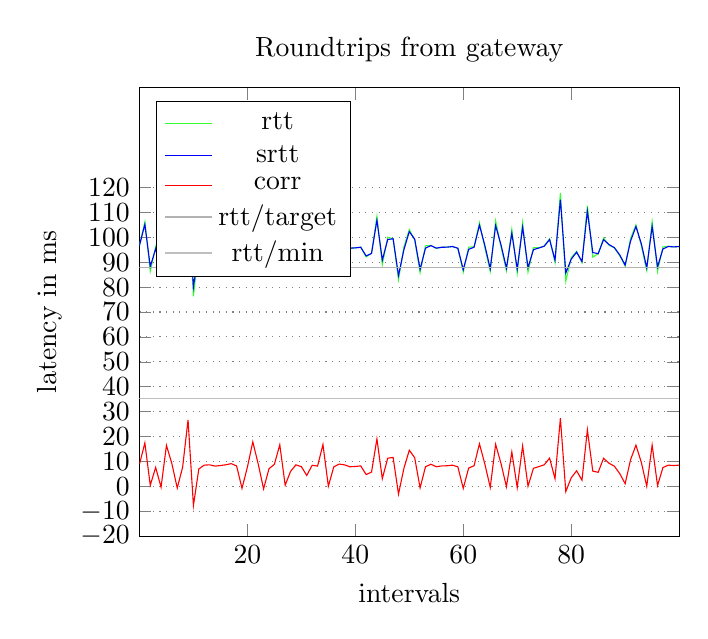
\begin{tikzpicture}\begin{axis}[
title={Roundtrips from gateway},
xlabel={intervals}, ylabel={latency in ms},
xmin=0, xmax=700,ymin=-20, ymax=160,
xtick={100,200,300,400,500,600},
xmin=000, xmax=100,ymin=-20, ymax=160,
xtick={20,40,60,80},
ytick={-40,-30,-20,-10,0,10,20,30,40,50,60,70,80,90,100,110,120},
legend pos=north west, grid style={dotted,gray},ymajorgrids=true,]
\addplot[ color=green!80 ] coordinates {(0,96.81)(1,106.145)(2,86.362)(3,96.163)(4,86.605)(5,106.091)(6,96.151)(7,86.003)(8,96.455)(9,116.585)(10,76.299)(11,96.416)(12,96.475)(13,96.448)(14,95.856)(15,96.169)(16,96.478)(17,96.966)(18,95.875)(19,85.998)(20,96.457)(21,106.789)(22,95.827)(23,85.653)(24,95.76)(25,96.826)(26,105.36)(27,86.432)(28,94.43)(29,96.721)(30,95.607)(31,91.784)(32,96.713)(33,95.865)(34,105.551)(35,85.983)(36,96.441)(37,96.87)(38,96.377)(39,95.571)(40,95.777)(41,96.038)(42,92.144)(43,93.616)(44,108.322)(45,89.097)(46,100.015)(47,99.447)(48,83.061)(49,96.161)(50,103.101)(51,98.946)(52,85.831)(53,96.571)(54,96.781)(55,95.548)(56,96.026)(57,96.066)(58,96.321)(59,95.548)(60,86.038)(61,96.056)(62,96.142)(63,105.87)(64,95.848)(65,86.347)(66,106.594)(67,96.06)(68,86.594)(69,103.156)(70,85.709)(71,105.883)(72,86.043)(73,95.82)(74,95.787)(75,96.503)(76,99.42)(77,89.945)(78,117.855)(79,82.417)(80,91.8)(81,94.355)(82,89.851)(83,112.73)(84,92.064)(85,93.374)(86,99.692)(87,96.873)(88,95.747)(89,92.576)(90,88.411)(91,99.555)(92,104.966)(93,96.627)(94,86.729)(95,106.205)(96,86.31)(97,96.122)(98,96.42)(99,96.135)(100,96.324)};\addlegendentry{rtt}
\addplot[ color=blue ] coordinates {(0,96.714001526)(1,105.201900153)(2,88.2459900153)(3,95.3712990015)(4,87.4816299002)(5,104.23006299)(6,96.958906299)(7,87.0985906299)(8,95.519359063)(9,114.478435906)(10,80.1169435906)(11,94.7860943591)(12,96.3061094359)(13,96.4338109436)(14,95.9137810944)(15,96.1434781094)(16,96.4445478109)(17,96.9138547811)(18,95.9788854781)(19,86.9960885478)(20,95.5109088548)(21,105.661190885)(22,96.8104190885)(23,86.7687419089)(24,94.8608741909)(25,96.6294874191)(26,104.486948742)(27,88.2374948742)(28,93.8107494874)(29,96.4299749487)(30,95.6892974949)(31,92.1745297495)(32,96.2591529749)(33,95.9044152975)(34,104.58634153)(35,87.843334153)(36,95.5812334153)(37,96.7411233415)(38,96.4134123342)(39,95.6552412334)(40,95.7648241233)(41,96.0106824123)(42,92.5306682412)(43,93.5074668241)(44,106.840546682)(45,90.8713546682)(46,99.1006354668)(47,99.4123635467)(48,84.6961363547)(49,95.0145136355)(50,102.292351364)(51,99.2806351364)(52,87.1759635136)(53,95.6314963514)(54,96.6660496351)(55,95.6598049635)(56,95.9893804964)(57,96.0583380496)(58,96.294733805)(59,95.6226733805)(60,86.996467338)(61,95.1500467338)(62,96.0428046734)(63,104.887280467)(64,96.7519280467)(65,87.3874928047)(66,104.67334928)(67,96.921334928)(68,87.6267334928)(69,101.603073349)(70,87.2984073349)(71,104.024540733)(72,87.8411540733)(73,95.0221154073)(74,95.7105115407)(75,96.4237511541)(76,99.1203751154)(77,90.8625375115)(78,115.155753751)(79,85.6908753751)(80,91.1890875375)(81,94.0384087538)(82,90.2697408754)(83,110.483974088)(84,93.9059974088)(85,93.4271997409)(86,99.0655199741)(87,97.0922519974)(88,95.8815251997)(89,92.90655252)(90,88.860555252)(91,98.4855555252)(92,104.317955553)(93,97.3960955553)(94,87.7957095555)(95,104.364070956)(96,88.1154070956)(97,95.3213407096)(98,96.310134071)(99,96.1525134071)(100,96.3068513407)};\addlegendentry{srtt}
\addplot[ color=red ] coordinates {(0,8.936501526)(1,17.4244001526)(2,0.46849001526)(3,7.59379900153)(4,-0.295870099847)(5,16.45256299)(6,9.181406299)(7,-0.6789093701)(8,7.74185906299)(9,26.7009359063)(10,-7.66055640937)(11,7.00859435906)(12,8.52860943591)(13,8.65631094359)(14,8.13628109436)(15,8.36597810944)(16,8.66704781094)(17,9.13635478109)(18,8.20138547811)(19,-0.781411452189)(20,7.73340885478)(21,17.8836908855)(22,9.03291908855)(23,-1.00875809115)(24,7.08337419089)(25,8.85198741909)(26,16.7094487419)(27,0.459994874191)(28,6.03324948742)(29,8.65247494874)(30,7.91179749487)(31,4.39702974949)(32,8.48165297495)(33,8.12691529749)(34,16.8088415297)(35,0.065834152975)(36,7.8037334153)(37,8.96362334153)(38,8.63591233415)(39,7.87774123342)(40,7.98732412334)(41,8.23318241233)(42,4.75316824123)(43,5.72996682412)(44,19.0630466824)(45,3.09385466824)(46,11.3231354668)(47,11.6348635467)(48,-3.08136364533)(49,7.23701363547)(50,14.5148513635)(51,11.5031351364)(52,-0.601536486365)(53,7.85399635136)(54,8.88854963514)(55,7.88230496351)(56,8.21188049635)(57,8.28083804964)(58,8.51723380496)(59,7.8451733805)(60,-0.78103266195)(61,7.3725467338)(62,8.26530467338)(63,17.1097804673)(64,8.97442804673)(65,-0.390007195327)(66,16.8958492805)(67,9.14383492805)(68,-0.150766507195)(69,13.8255733493)(70,-0.479092665072)(71,16.2470407335)(72,0.0636540733493)(73,7.24461540733)(74,7.93301154073)(75,8.64625115407)(76,11.3428751154)(77,3.08503751154)(78,27.3782537512)(79,-2.08662462488)(80,3.41158753751)(81,6.26090875375)(82,2.49224087538)(83,22.7064740875)(84,6.12849740875)(85,5.64969974088)(86,11.2880199741)(87,9.31475199741)(88,8.10402519974)(89,5.12905251997)(90,1.083055252)(91,10.7080555252)(92,16.5404555525)(93,9.61859555525)(94,0.0182095555252)(95,16.5865709556)(96,0.337907095555)(97,7.54384070956)(98,8.53263407096)(99,8.3750134071)(100,8.52935134071)};\addlegendentry{corr}
\addplot[ color=gray!60 ] coordinates {(0,87.7775)(1,87.7775)(2,87.7775)(3,87.7775)(4,87.7775)(5,87.7775)(6,87.7775)(7,87.7775)(8,87.7775)(9,87.7775)(10,87.7775)(11,87.7775)(12,87.7775)(13,87.7775)(14,87.7775)(15,87.7775)(16,87.7775)(17,87.7775)(18,87.7775)(19,87.7775)(20,87.7775)(21,87.7775)(22,87.7775)(23,87.7775)(24,87.7775)(25,87.7775)(26,87.7775)(27,87.7775)(28,87.7775)(29,87.7775)(30,87.7775)(31,87.7775)(32,87.7775)(33,87.7775)(34,87.7775)(35,87.7775)(36,87.7775)(37,87.7775)(38,87.7775)(39,87.7775)(40,87.7775)(41,87.7775)(42,87.7775)(43,87.7775)(44,87.7775)(45,87.7775)(46,87.7775)(47,87.7775)(48,87.7775)(49,87.7775)(50,87.7775)(51,87.7775)(52,87.7775)(53,87.7775)(54,87.7775)(55,87.7775)(56,87.7775)(57,87.7775)(58,87.7775)(59,87.7775)(60,87.7775)(61,87.7775)(62,87.7775)(63,87.7775)(64,87.7775)(65,87.7775)(66,87.7775)(67,87.7775)(68,87.7775)(69,87.7775)(70,87.7775)(71,87.7775)(72,87.7775)(73,87.7775)(74,87.7775)(75,87.7775)(76,87.7775)(77,87.7775)(78,87.7775)(79,87.7775)(80,87.7775)(81,87.7775)(82,87.7775)(83,87.7775)(84,87.7775)(85,87.7775)(86,87.7775)(87,87.7775)(88,87.7775)(89,87.7775)(90,87.7775)(91,87.7775)(92,87.7775)(93,87.7775)(94,87.7775)(95,87.7775)(96,87.7775)(97,87.7775)(98,87.7775)(99,87.7775)(100,87.7775)};\addlegendentry{rtt/target}
\addplot[ color=gray!50  ] coordinates {(0,35.111)(1,35.111)(2,35.111)(3,35.111)(4,35.111)(5,35.111)(6,35.111)(7,35.111)(8,35.111)(9,35.111)(10,35.111)(11,35.111)(12,35.111)(13,35.111)(14,35.111)(15,35.111)(16,35.111)(17,35.111)(18,35.111)(19,35.111)(20,35.111)(21,35.111)(22,35.111)(23,35.111)(24,35.111)(25,35.111)(26,35.111)(27,35.111)(28,35.111)(29,35.111)(30,35.111)(31,35.111)(32,35.111)(33,35.111)(34,35.111)(35,35.111)(36,35.111)(37,35.111)(38,35.111)(39,35.111)(40,35.111)(41,35.111)(42,35.111)(43,35.111)(44,35.111)(45,35.111)(46,35.111)(47,35.111)(48,35.111)(49,35.111)(50,35.111)(51,35.111)(52,35.111)(53,35.111)(54,35.111)(55,35.111)(56,35.111)(57,35.111)(58,35.111)(59,35.111)(60,35.111)(61,35.111)(62,35.111)(63,35.111)(64,35.111)(65,35.111)(66,35.111)(67,35.111)(68,35.111)(69,35.111)(70,35.111)(71,35.111)(72,35.111)(73,35.111)(74,35.111)(75,35.111)(76,35.111)(77,35.111)(78,35.111)(79,35.111)(80,35.111)(81,35.111)(82,35.111)(83,35.111)(84,35.111)(85,35.111)(86,35.111)(87,35.111)(88,35.111)(89,35.111)(90,35.111)(91,35.111)(92,35.111)(93,35.111)(94,35.111)(95,35.111)(96,35.111)(97,35.111)(98,35.111)(99,35.111)(100,35.111)};\addlegendentry{rtt/min}
\end{axis}\end{tikzpicture}
\caption{gw/test/alpha/0.9/rtttarget/2.5/diff/1.0/slope/0.15/zommed}
\label{fig:gw/test/alpha/0.9/rtttarget/2.5/diff/1.0/slope/0.15/zommed}
\end{figure}

\begin{figure}\centering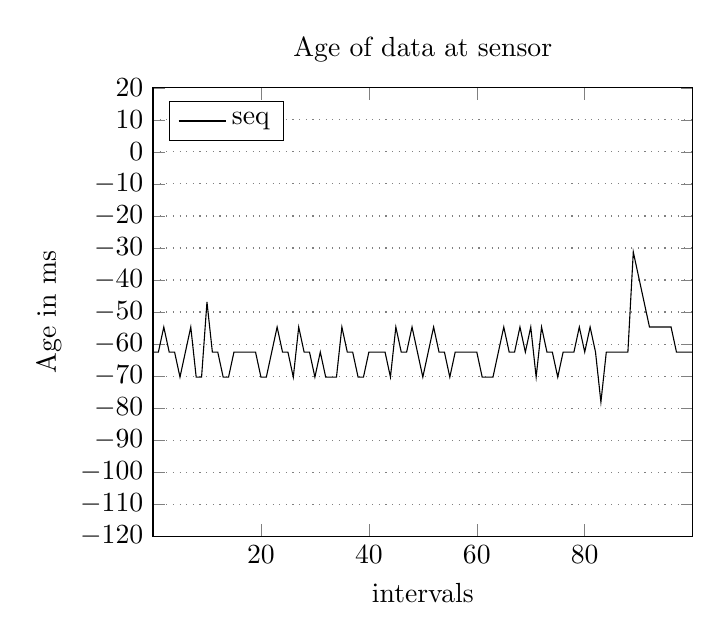
\begin{tikzpicture}\begin{axis}[
title={Age of data at sensor},
xlabel={intervals}, ylabel={Age in ms},
xmin=000, xmax=100,ymin=-120, ymax=20,
xtick={20,40,60,80},
ytick={-120,-110, -100,-90,-80,-70,-60,-50,-40,-30,-20,-10,0,10,20},
legend pos=north west, grid style={dotted,gray},ymajorgrids=true,]
\addplot[  ] coordinates {(0,-62.5)(1,-62.5)(2,-54.6875)(3,-62.5)(4,-62.5)(5,-70.3125)(6,-62.5)(7,-54.6875)(8,-70.3125)(9,-70.3125)(10,-46.875)(11,-62.5)(12,-62.5)(13,-70.3125)(14,-70.3125)(15,-62.5)(16,-62.5)(17,-62.5)(18,-62.5)(19,-62.5)(20,-70.3125)(21,-70.3125)(22,-62.5)(23,-54.6875)(24,-62.5)(25,-62.5)(26,-70.3125)(27,-54.6875)(28,-62.5)(29,-62.5)(30,-70.3125)(31,-62.5)(32,-70.3125)(33,-70.3125)(34,-70.3125)(35,-54.6875)(36,-62.5)(37,-62.5)(38,-70.3125)(39,-70.3125)(40,-62.5)(41,-62.5)(42,-62.5)(43,-62.5)(44,-70.3125)(45,-54.6875)(46,-62.5)(47,-62.5)(48,-54.6875)(49,-62.5)(50,-70.3125)(51,-62.5)(52,-54.6875)(53,-62.5)(54,-62.5)(55,-70.3125)(56,-62.5)(57,-62.5)(58,-62.5)(59,-62.5)(60,-62.5)(61,-70.3125)(62,-70.3125)(63,-70.3125)(64,-62.5)(65,-54.6875)(66,-62.5)(67,-62.5)(68,-54.6875)(69,-62.5)(70,-54.6875)(71,-70.3125)(72,-54.6875)(73,-62.5)(74,-62.5)(75,-70.3125)(76,-62.5)(77,-62.5)(78,-62.5)(79,-54.6875)(80,-62.5)(81,-54.6875)(82,-62.5)(83,-78.125)(84,-62.5)(85,-62.5)(86,-62.5)(87,-62.5)(88,-62.5)(89,-31.25)(90,-39.0625)(91,-46.875)(92,-54.6875)(93,-54.6875)(94,-54.6875)(95,-54.6875)(96,-54.6875)(97,-62.5)(98,-62.5)(99,-62.5)(100,-62.5)};\addlegendentry{seq}
\end{axis}\end{tikzpicture}
\caption{sensor/test/alpha/0.9/rtttarget/2.5/diff/1.0/slope/0.15/zommed}
\label{fig:sensor/test/alpha/0.9/rtttarget/2.5/diff/1.0/slope/0.15/zommed}
\end{figure}


%%%%%%


\begin{figure}\centering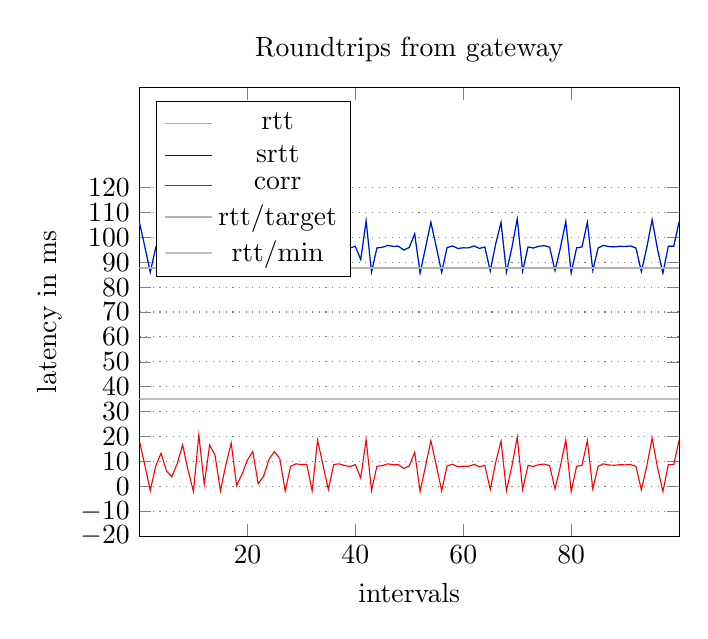
\begin{tikzpicture}\begin{axis}[
title={Roundtrips from gateway},
xlabel={intervals}, ylabel={latency in ms},
xmin=0, xmax=700,ymin=-20, ymax=160,
xtick={100,200,300,400,500,600},
xmin=000, xmax=100,ymin=-20, ymax=160,
xtick={20,40,60,80},
ytick={-40,-30,-20,-10,0,10,20,30,40,50,60,70,80,90,100,110,120},
legend pos=north west, grid style={dotted,gray},ymajorgrids=true,]
\addplot[ color=green!80 ] coordinates {(0,105.879)(1,96.132)(2,85.98)(3,95.793)(4,101.006)(5,93.881)(6,91.594)(7,96.865)(8,104.351)(9,94.164)(10,85.671)(11,108.376)(12,88.504)(13,104.288)(14,100.292)(15,85.885)(16,96.287)(17,105.052)(18,88.112)(19,92.496)(20,98.286)(21,101.694)(22,88.783)(23,91.762)(24,98.552)(25,101.689)(26,98.886)(27,85.802)(28,95.739)(29,96.744)(30,96.448)(31,96.527)(32,85.973)(33,106.206)(34,96.354)(35,86.413)(36,96.481)(37,96.744)(38,96.049)(39,95.698)(40,96.404)(41,91.066)(42,106.536)(43,86.027)(44,95.757)(45,96.001)(46,96.745)(47,96.389)(48,96.392)(49,94.88)(50,95.927)(51,101.384)(52,85.652)(53,95.726)(54,106.055)(55,96.174)(56,85.946)(57,95.857)(58,96.544)(59,95.512)(60,95.794)(61,95.772)(62,96.514)(63,95.545)(64,96.108)(65,86.458)(66,97.255)(67,105.929)(68,86.005)(69,95.704)(70,107.455)(71,86.438)(72,96.099)(73,95.703)(74,96.415)(75,96.644)(76,96.071)(77,86.651)(78,95.753)(79,106.385)(80,85.659)(81,95.777)(82,96.12)(83,106.077)(84,86.739)(85,95.78)(86,96.74)(87,96.28)(88,96.178)(89,96.402)(90,96.343)(91,96.521)(92,95.693)(93,86.278)(94,95.775)(95,107.07)(96,95.149)(97,85.66)(98,96.406)(99,96.408)(100,106.175)};\addlegendentry{rtt}
\addplot[ color=blue ] coordinates {(0,105.879)(1,96.132)(2,85.98)(3,95.793)(4,101.006)(5,93.881)(6,91.594)(7,96.865)(8,104.351)(9,94.164)(10,85.671)(11,108.376)(12,88.504)(13,104.288)(14,100.292)(15,85.885)(16,96.287)(17,105.052)(18,88.112)(19,92.496)(20,98.286)(21,101.694)(22,88.783)(23,91.762)(24,98.552)(25,101.689)(26,98.886)(27,85.802)(28,95.739)(29,96.744)(30,96.448)(31,96.527)(32,85.973)(33,106.206)(34,96.354)(35,86.413)(36,96.481)(37,96.744)(38,96.049)(39,95.698)(40,96.404)(41,91.066)(42,106.536)(43,86.027)(44,95.757)(45,96.001)(46,96.745)(47,96.389)(48,96.392)(49,94.88)(50,95.927)(51,101.384)(52,85.652)(53,95.726)(54,106.055)(55,96.174)(56,85.946)(57,95.857)(58,96.544)(59,95.512)(60,95.794)(61,95.772)(62,96.514)(63,95.545)(64,96.108)(65,86.458)(66,97.255)(67,105.929)(68,86.005)(69,95.704)(70,107.455)(71,86.438)(72,96.099)(73,95.703)(74,96.415)(75,96.644)(76,96.071)(77,86.651)(78,95.753)(79,106.385)(80,85.659)(81,95.777)(82,96.12)(83,106.077)(84,86.739)(85,95.78)(86,96.74)(87,96.28)(88,96.178)(89,96.402)(90,96.343)(91,96.521)(92,95.693)(93,86.278)(94,95.775)(95,107.07)(96,95.149)(97,85.66)(98,96.406)(99,96.408)(100,106.175)};\addlegendentry{srtt}
\addplot[ color=red ] coordinates {(0,18.1865)(1,8.4395)(2,-1.7125)(3,8.1005)(4,13.3135)(5,6.1885)(6,3.9015)(7,9.1725)(8,16.6585)(9,6.4715)(10,-2.0215)(11,20.6835)(12,0.8115)(13,16.5955)(14,12.5995)(15,-1.8075)(16,8.5945)(17,17.3595)(18,0.4195)(19,4.8035)(20,10.5935)(21,14.0015)(22,1.0905)(23,4.0695)(24,10.8595)(25,13.9965)(26,11.1935)(27,-1.8905)(28,8.0465)(29,9.0515)(30,8.7555)(31,8.8345)(32,-1.7195)(33,18.5135)(34,8.6615)(35,-1.2795)(36,8.7885)(37,9.0515)(38,8.3565)(39,8.0055)(40,8.7115)(41,3.3735)(42,18.8435)(43,-1.6655)(44,8.0645)(45,8.3085)(46,9.0525)(47,8.6965)(48,8.6995)(49,7.1875)(50,8.2345)(51,13.6915)(52,-2.0405)(53,8.0335)(54,18.3625)(55,8.4815)(56,-1.7465)(57,8.1645)(58,8.8515)(59,7.8195)(60,8.1015)(61,8.0795)(62,8.8215)(63,7.8525)(64,8.4155)(65,-1.2345)(66,9.5625)(67,18.2365)(68,-1.6875)(69,8.0115)(70,19.7625)(71,-1.2545)(72,8.4065)(73,8.0105)(74,8.7225)(75,8.9515)(76,8.3785)(77,-1.0415)(78,8.0605)(79,18.6925)(80,-2.0335)(81,8.0845)(82,8.4275)(83,18.3845)(84,-0.9535)(85,8.0875)(86,9.0475)(87,8.5875)(88,8.4855)(89,8.7095)(90,8.6505)(91,8.8285)(92,8.0005)(93,-1.4145)(94,8.0825)(95,19.3775)(96,7.4565)(97,-2.0325)(98,8.7135)(99,8.7155)(100,18.4825)};\addlegendentry{corr}
\addplot[ color=gray!60 ] coordinates {(0,87.6925)(1,87.6925)(2,87.6925)(3,87.6925)(4,87.6925)(5,87.6925)(6,87.6925)(7,87.6925)(8,87.6925)(9,87.6925)(10,87.6925)(11,87.6925)(12,87.6925)(13,87.6925)(14,87.6925)(15,87.6925)(16,87.6925)(17,87.6925)(18,87.6925)(19,87.6925)(20,87.6925)(21,87.6925)(22,87.6925)(23,87.6925)(24,87.6925)(25,87.6925)(26,87.6925)(27,87.6925)(28,87.6925)(29,87.6925)(30,87.6925)(31,87.6925)(32,87.6925)(33,87.6925)(34,87.6925)(35,87.6925)(36,87.6925)(37,87.6925)(38,87.6925)(39,87.6925)(40,87.6925)(41,87.6925)(42,87.6925)(43,87.6925)(44,87.6925)(45,87.6925)(46,87.6925)(47,87.6925)(48,87.6925)(49,87.6925)(50,87.6925)(51,87.6925)(52,87.6925)(53,87.6925)(54,87.6925)(55,87.6925)(56,87.6925)(57,87.6925)(58,87.6925)(59,87.6925)(60,87.6925)(61,87.6925)(62,87.6925)(63,87.6925)(64,87.6925)(65,87.6925)(66,87.6925)(67,87.6925)(68,87.6925)(69,87.6925)(70,87.6925)(71,87.6925)(72,87.6925)(73,87.6925)(74,87.6925)(75,87.6925)(76,87.6925)(77,87.6925)(78,87.6925)(79,87.6925)(80,87.6925)(81,87.6925)(82,87.6925)(83,87.6925)(84,87.6925)(85,87.6925)(86,87.6925)(87,87.6925)(88,87.6925)(89,87.6925)(90,87.6925)(91,87.6925)(92,87.6925)(93,87.6925)(94,87.6925)(95,87.6925)(96,87.6925)(97,87.6925)(98,87.6925)(99,87.6925)(100,87.6925)};\addlegendentry{rtt/target}
\addplot[ color=gray!50  ] coordinates {(0,35.077)(1,35.077)(2,35.077)(3,35.077)(4,35.077)(5,35.077)(6,35.077)(7,35.077)(8,35.077)(9,35.077)(10,35.077)(11,35.077)(12,35.077)(13,35.077)(14,35.077)(15,35.077)(16,35.077)(17,35.077)(18,35.077)(19,35.077)(20,35.077)(21,35.077)(22,35.077)(23,35.077)(24,35.077)(25,35.077)(26,35.077)(27,35.077)(28,35.077)(29,35.077)(30,35.077)(31,35.077)(32,35.077)(33,35.077)(34,35.077)(35,35.077)(36,35.077)(37,35.077)(38,35.077)(39,35.077)(40,35.077)(41,35.077)(42,35.077)(43,35.077)(44,35.077)(45,35.077)(46,35.077)(47,35.077)(48,35.077)(49,35.077)(50,35.077)(51,35.077)(52,35.077)(53,35.077)(54,35.077)(55,35.077)(56,35.077)(57,35.077)(58,35.077)(59,35.077)(60,35.077)(61,35.077)(62,35.077)(63,35.077)(64,35.077)(65,35.077)(66,35.077)(67,35.077)(68,35.077)(69,35.077)(70,35.077)(71,35.077)(72,35.077)(73,35.077)(74,35.077)(75,35.077)(76,35.077)(77,35.077)(78,35.077)(79,35.077)(80,35.077)(81,35.077)(82,35.077)(83,35.077)(84,35.077)(85,35.077)(86,35.077)(87,35.077)(88,35.077)(89,35.077)(90,35.077)(91,35.077)(92,35.077)(93,35.077)(94,35.077)(95,35.077)(96,35.077)(97,35.077)(98,35.077)(99,35.077)(100,35.077)};\addlegendentry{rtt/min}
\end{axis}\end{tikzpicture}
\caption{gw/test/alpha/1.0/rtttarget/2.5/diff/1.0/slope/0.15/zommed}
\label{fig:gw/test/alpha/1.0/rtttarget/2.5/diff/1.0/slope/0.15/zommed}
\end{figure}

\begin{figure}\centering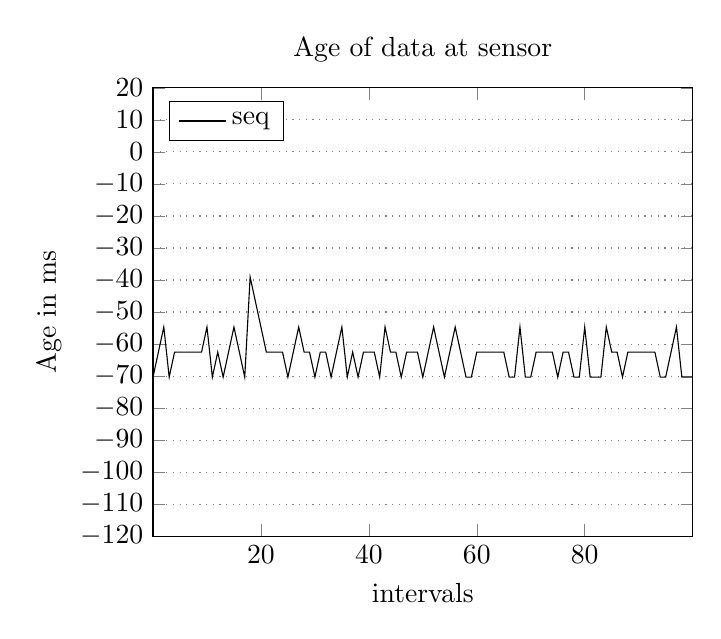
\begin{tikzpicture}\begin{axis}[
title={Age of data at sensor},
xlabel={intervals}, ylabel={Age in ms},
xmin=000, xmax=100,ymin=-120, ymax=20,
xtick={20,40,60,80},
ytick={-120,-110, -100,-90,-80,-70,-60,-50,-40,-30,-20,-10,0,10,20},
legend pos=north west, grid style={dotted,gray},ymajorgrids=true,]
\addplot[  ] coordinates {(0,-70.3125)(1,-62.5)(2,-54.6875)(3,-70.3125)(4,-62.5)(5,-62.5)(6,-62.5)(7,-62.5)(8,-62.5)(9,-62.5)(10,-54.6875)(11,-70.3125)(12,-62.5)(13,-70.3125)(14,-62.5)(15,-54.6875)(16,-62.5)(17,-70.3125)(18,-39.0625)(19,-46.875)(20,-54.6875)(21,-62.5)(22,-62.5)(23,-62.5)(24,-62.5)(25,-70.3125)(26,-62.5)(27,-54.6875)(28,-62.5)(29,-62.5)(30,-70.3125)(31,-62.5)(32,-62.5)(33,-70.3125)(34,-62.5)(35,-54.6875)(36,-70.3125)(37,-62.5)(38,-70.3125)(39,-62.5)(40,-62.5)(41,-62.5)(42,-70.3125)(43,-54.6875)(44,-62.5)(45,-62.5)(46,-70.3125)(47,-62.5)(48,-62.5)(49,-62.5)(50,-70.3125)(51,-62.5)(52,-54.6875)(53,-62.5)(54,-70.3125)(55,-62.5)(56,-54.6875)(57,-62.5)(58,-70.3125)(59,-70.3125)(60,-62.5)(61,-62.5)(62,-62.5)(63,-62.5)(64,-62.5)(65,-62.5)(66,-70.3125)(67,-70.3125)(68,-54.6875)(69,-70.3125)(70,-70.3125)(71,-62.5)(72,-62.5)(73,-62.5)(74,-62.5)(75,-70.3125)(76,-62.5)(77,-62.5)(78,-70.3125)(79,-70.3125)(80,-54.6875)(81,-70.3125)(82,-70.3125)(83,-70.3125)(84,-54.6875)(85,-62.5)(86,-62.5)(87,-70.3125)(88,-62.5)(89,-62.5)(90,-62.5)(91,-62.5)(92,-62.5)(93,-62.5)(94,-70.3125)(95,-70.3125)(96,-62.5)(97,-54.6875)(98,-70.3125)(99,-70.3125)(100,-70.3125)};\addlegendentry{seq}
\end{axis}\end{tikzpicture}
\caption{sensor/test/alpha/1.0/rtttarget/2.5/diff/1.0/slope/0.15/zommed}
\label{fig:sensor/test/alpha/1.0/rtttarget/2.5/diff/1.0/slope/0.15/zommed}
\end{figure}

%%%%%%%%%%%

%%%%%%%%%%%


\begin{figure}\centering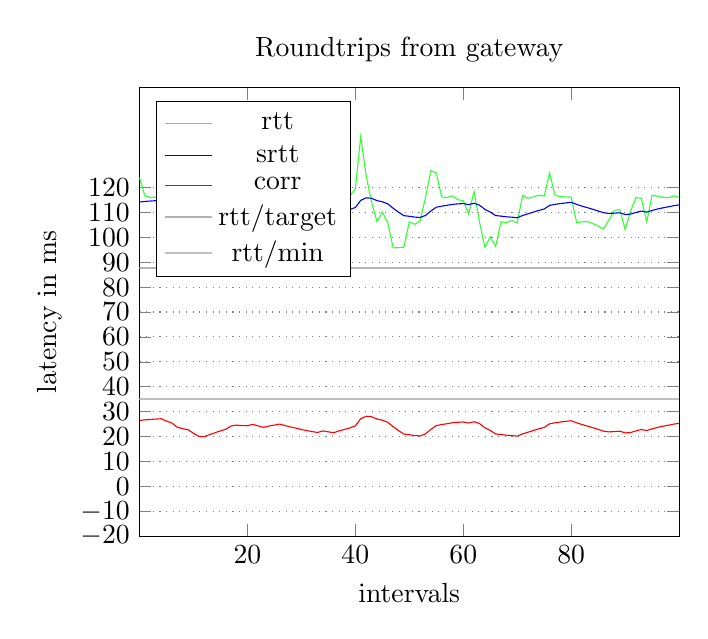
\begin{tikzpicture}\begin{axis}[
title={Roundtrips from gateway},
xlabel={intervals}, ylabel={latency in ms},
xmin=0, xmax=700,ymin=-20, ymax=160,
xtick={100,200,300,400,500,600},
xmin=000, xmax=100,ymin=-20, ymax=160,
xtick={20,40,60,80},
ytick={-40,-30,-20,-10,0,10,20,30,40,50,60,70,80,90,100,110,120},
legend pos=north west, grid style={dotted,gray},ymajorgrids=true,]
\addplot[ color=green!80 ] coordinates {(0,124.012)(1,116.638)(2,116.009)(3,116.098)(4,116.038)(5,105.872)(6,105.82)(7,96.14)(8,105.991)(9,106.233)(10,96.416)(11,96.483)(12,106.477)(13,116.017)(14,115.931)(15,116.734)(16,116.579)(17,124.073)(18,114.971)(19,110.694)(20,111.434)(21,117.424)(22,106.475)(23,105.864)(24,116.9)(25,115.67)(26,116.429)(27,106.516)(28,106.647)(29,106.871)(30,105.747)(31,105.826)(32,106.204)(33,106.174)(34,115.658)(35,106.107)(36,106.294)(37,116.593)(38,115.68)(39,116.692)(40,119.421)(41,140.496)(42,124.756)(43,114.265)(44,106.315)(45,110.071)(46,105.999)(47,95.766)(48,95.836)(49,96.031)(50,106.208)(51,105.243)(52,106.55)(53,115.972)(54,126.789)(55,125.768)(56,116.254)(57,115.949)(58,116.68)(59,115.078)(60,114.726)(61,109.295)(62,118.469)(63,106.276)(64,96.098)(65,100.199)(66,96.303)(67,106.252)(68,105.861)(69,106.684)(70,105.803)(71,116.837)(72,115.673)(73,116.254)(74,116.9)(75,116.596)(76,125.759)(77,116.947)(78,116.292)(79,116.232)(80,116.151)(81,105.895)(82,106.192)(83,106.324)(84,105.497)(85,104.476)(86,103.419)(87,106.937)(88,110.824)(89,111.159)(90,103.105)(91,110.563)(92,115.959)(93,115.616)(94,106.271)(95,116.934)(96,116.516)(97,116.02)(98,115.927)(99,116.648)(100,116.078)};\addlegendentry{rtt}
\addplot[ color=blue ] coordinates {(0,114.152379206)(1,114.400941286)(2,114.561747157)(3,114.715372441)(4,114.847635197)(5,113.950071677)(6,113.13706451)(7,111.437358059)(8,110.892722253)(9,110.426750028)(10,109.025675025)(11,107.771407522)(12,107.64196677)(13,108.479470093)(14,109.224623084)(15,109.975560775)(16,110.635904698)(17,111.979614228)(18,112.278752805)(19,112.120277525)(20,112.051649772)(21,112.588884795)(22,111.977496316)(23,111.366146684)(24,111.919532016)(25,112.294578814)(26,112.708020933)(27,112.088818839)(28,111.544636955)(29,111.07727326)(30,110.544245934)(31,110.072421341)(32,109.685579206)(33,109.334421286)(34,109.966779157)(35,109.580801242)(36,109.252121117)(37,109.986209006)(38,110.555588105)(39,111.169229295)(40,111.994406365)(41,114.844565729)(42,115.835709156)(43,115.67863824)(44,114.742274416)(45,114.275146975)(46,113.447532277)(47,111.679379049)(48,110.095041144)(49,108.68863703)(50,108.440573327)(51,108.120815994)(52,107.963734395)(53,108.764560955)(54,110.56700486)(55,112.087104374)(56,112.503793936)(57,112.848314543)(58,113.231483089)(59,113.41613478)(60,113.547121302)(61,113.121909172)(62,113.656618254)(63,112.918556429)(64,111.236500786)(65,110.132750707)(66,108.749775637)(67,108.499998073)(68,108.236098266)(69,108.080888439)(70,107.853099595)(71,108.751489636)(72,109.443640672)(73,110.124676605)(74,110.802208944)(75,111.38158805)(76,112.819329245)(77,113.23209632)(78,113.538086688)(79,113.80747802)(80,114.041830218)(81,113.227147196)(82,112.523632476)(83,111.903669229)(84,111.263002306)(85,110.584302075)(86,109.867771868)(87,109.574694681)(88,109.699625213)(89,109.845562692)(90,109.171506422)(91,109.31065578)(92,109.975490202)(93,110.539541182)(94,110.112687064)(95,110.794818357)(96,111.366936522)(97,111.832242869)(98,112.241718583)(99,112.682346724)(100,113.021912052)};\addlegendentry{srtt}
\addplot[ color=red ] coordinates {(0,26.4598792062)(1,26.7084412856)(2,26.869247157)(3,27.0228724413)(4,27.1551351972)(5,26.2575716775)(6,25.4445645097)(7,23.7448580587)(8,23.2002222529)(9,22.7342500276)(10,21.3331750248)(11,20.0789075223)(12,19.9494667701)(13,20.7869700931)(14,21.5321230838)(15,22.2830607754)(16,22.9434046979)(17,24.2871142281)(18,24.5862528053)(19,24.4277775247)(20,24.3591497723)(21,24.896384795)(22,24.2849963155)(23,23.673646684)(24,24.2270320156)(25,24.602078814)(26,25.0155209326)(27,24.3963188394)(28,23.8521369554)(29,23.3847732599)(30,22.8517459339)(31,22.3799213405)(32,21.9930792065)(33,21.6419212858)(34,22.2742791572)(35,21.8883012415)(36,21.5596211174)(37,22.2937090056)(38,22.8630881051)(39,23.4767292946)(40,24.3019063651)(41,27.1520657286)(42,28.1432091557)(43,27.9861382402)(44,27.0497744161)(45,26.5826469745)(46,25.7550322771)(47,23.9868790494)(48,22.4025411444)(49,20.99613703)(50,20.748073327)(51,20.4283159943)(52,20.2712343949)(53,21.0720609554)(54,22.8745048598)(55,24.3946043739)(56,24.8112939365)(57,25.1558145428)(58,25.5389830885)(59,25.7236347797)(60,25.8546213017)(61,25.4294091715)(62,25.9641182544)(63,25.226056429)(64,23.5440007861)(65,22.4402507075)(66,21.0572756367)(67,20.807498073)(68,20.5435982657)(69,20.3883884392)(70,20.1605995952)(71,21.0589896357)(72,21.7511406721)(73,22.4321766049)(74,23.1097089444)(75,23.68908805)(76,25.126829245)(77,25.5395963205)(78,25.8455866884)(79,26.1149780196)(80,26.3493302176)(81,25.5346471959)(82,24.8311324763)(83,24.2111692287)(84,23.5705023058)(85,22.8918020752)(86,22.1752718677)(87,21.8821946809)(88,22.0071252128)(89,22.1530626915)(90,21.4790064224)(91,21.6181557802)(92,22.2829902021)(93,22.8470411819)(94,22.4201870637)(95,23.1023183574)(96,23.6744365216)(97,24.1397428695)(98,24.5492185825)(99,24.9898467243)(100,25.3294120518)};\addlegendentry{corr}
\addplot[ color=gray!60 ] coordinates {(0,87.6925)(1,87.6925)(2,87.6925)(3,87.6925)(4,87.6925)(5,87.6925)(6,87.6925)(7,87.6925)(8,87.6925)(9,87.6925)(10,87.6925)(11,87.6925)(12,87.6925)(13,87.6925)(14,87.6925)(15,87.6925)(16,87.6925)(17,87.6925)(18,87.6925)(19,87.6925)(20,87.6925)(21,87.6925)(22,87.6925)(23,87.6925)(24,87.6925)(25,87.6925)(26,87.6925)(27,87.6925)(28,87.6925)(29,87.6925)(30,87.6925)(31,87.6925)(32,87.6925)(33,87.6925)(34,87.6925)(35,87.6925)(36,87.6925)(37,87.6925)(38,87.6925)(39,87.6925)(40,87.6925)(41,87.6925)(42,87.6925)(43,87.6925)(44,87.6925)(45,87.6925)(46,87.6925)(47,87.6925)(48,87.6925)(49,87.6925)(50,87.6925)(51,87.6925)(52,87.6925)(53,87.6925)(54,87.6925)(55,87.6925)(56,87.6925)(57,87.6925)(58,87.6925)(59,87.6925)(60,87.6925)(61,87.6925)(62,87.6925)(63,87.6925)(64,87.6925)(65,87.6925)(66,87.6925)(67,87.6925)(68,87.6925)(69,87.6925)(70,87.6925)(71,87.6925)(72,87.6925)(73,87.6925)(74,87.6925)(75,87.6925)(76,87.6925)(77,87.6925)(78,87.6925)(79,87.6925)(80,87.6925)(81,87.6925)(82,87.6925)(83,87.6925)(84,87.6925)(85,87.6925)(86,87.6925)(87,87.6925)(88,87.6925)(89,87.6925)(90,87.6925)(91,87.6925)(92,87.6925)(93,87.6925)(94,87.6925)(95,87.6925)(96,87.6925)(97,87.6925)(98,87.6925)(99,87.6925)(100,87.6925)};\addlegendentry{rtt/target}
\addplot[ color=gray!50  ] coordinates {(0,35.077)(1,35.077)(2,35.077)(3,35.077)(4,35.077)(5,35.077)(6,35.077)(7,35.077)(8,35.077)(9,35.077)(10,35.077)(11,35.077)(12,35.077)(13,35.077)(14,35.077)(15,35.077)(16,35.077)(17,35.077)(18,35.077)(19,35.077)(20,35.077)(21,35.077)(22,35.077)(23,35.077)(24,35.077)(25,35.077)(26,35.077)(27,35.077)(28,35.077)(29,35.077)(30,35.077)(31,35.077)(32,35.077)(33,35.077)(34,35.077)(35,35.077)(36,35.077)(37,35.077)(38,35.077)(39,35.077)(40,35.077)(41,35.077)(42,35.077)(43,35.077)(44,35.077)(45,35.077)(46,35.077)(47,35.077)(48,35.077)(49,35.077)(50,35.077)(51,35.077)(52,35.077)(53,35.077)(54,35.077)(55,35.077)(56,35.077)(57,35.077)(58,35.077)(59,35.077)(60,35.077)(61,35.077)(62,35.077)(63,35.077)(64,35.077)(65,35.077)(66,35.077)(67,35.077)(68,35.077)(69,35.077)(70,35.077)(71,35.077)(72,35.077)(73,35.077)(74,35.077)(75,35.077)(76,35.077)(77,35.077)(78,35.077)(79,35.077)(80,35.077)(81,35.077)(82,35.077)(83,35.077)(84,35.077)(85,35.077)(86,35.077)(87,35.077)(88,35.077)(89,35.077)(90,35.077)(91,35.077)(92,35.077)(93,35.077)(94,35.077)(95,35.077)(96,35.077)(97,35.077)(98,35.077)(99,35.077)(100,35.077)};\addlegendentry{rtt/min}
\end{axis}\end{tikzpicture}
\caption{gw/test/alpha/0.1/rtttarget/2.5/diff/1.02/slope/0.15/zommed}
\label{fig:gw/test/alpha/0.1/rtttarget/2.5/diff/1.02/slope/0.15/zommed}
\end{figure}



\begin{figure}\centering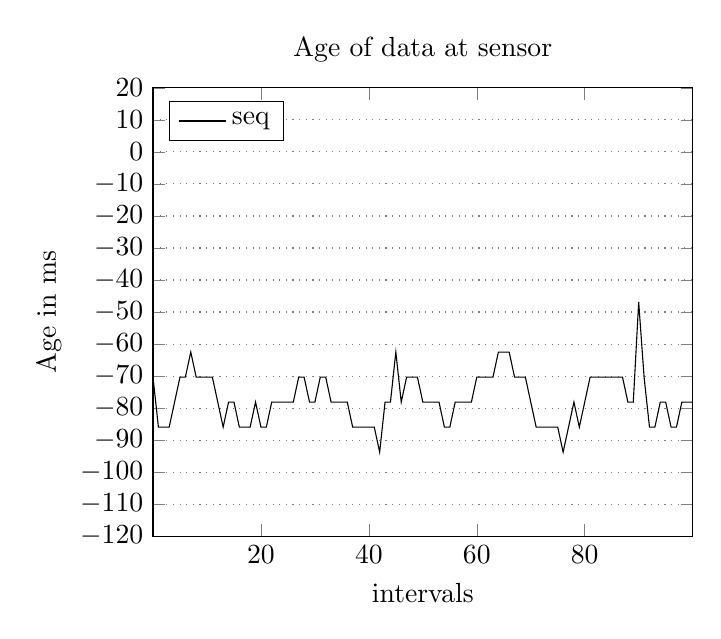
\begin{tikzpicture}\begin{axis}[
title={Age of data at sensor},
xlabel={intervals}, ylabel={Age in ms},
xmin=000, xmax=100,ymin=-120, ymax=20,
xtick={20,40,60,80},
ytick={-120,-110, -100,-90,-80,-70,-60,-50,-40,-30,-20,-10,0,10,20},
legend pos=north west, grid style={dotted,gray},ymajorgrids=true,]
\addplot[  ] coordinates {(0,-70.3125)(1,-85.9375)(2,-85.9375)(3,-85.9375)(4,-78.125)(5,-70.3125)(6,-70.3125)(7,-62.5)(8,-70.3125)(9,-70.3125)(10,-70.3125)(11,-70.3125)(12,-78.125)(13,-85.9375)(14,-78.125)(15,-78.125)(16,-85.9375)(17,-85.9375)(18,-85.9375)(19,-78.125)(20,-85.9375)(21,-85.9375)(22,-78.125)(23,-78.125)(24,-78.125)(25,-78.125)(26,-78.125)(27,-70.3125)(28,-70.3125)(29,-78.125)(30,-78.125)(31,-70.3125)(32,-70.3125)(33,-78.125)(34,-78.125)(35,-78.125)(36,-78.125)(37,-85.9375)(38,-85.9375)(39,-85.9375)(40,-85.9375)(41,-85.9375)(42,-93.75)(43,-78.125)(44,-78.125)(45,-62.5)(46,-78.125)(47,-70.3125)(48,-70.3125)(49,-70.3125)(50,-78.125)(51,-78.125)(52,-78.125)(53,-78.125)(54,-85.9375)(55,-85.9375)(56,-78.125)(57,-78.125)(58,-78.125)(59,-78.125)(60,-70.3125)(61,-70.3125)(62,-70.3125)(63,-70.3125)(64,-62.5)(65,-62.5)(66,-62.5)(67,-70.3125)(68,-70.3125)(69,-70.3125)(70,-78.125)(71,-85.9375)(72,-85.9375)(73,-85.9375)(74,-85.9375)(75,-85.9375)(76,-93.75)(77,-85.9375)(78,-78.125)(79,-85.9375)(80,-78.125)(81,-70.3125)(82,-70.3125)(83,-70.3125)(84,-70.3125)(85,-70.3125)(86,-70.3125)(87,-70.3125)(88,-78.125)(89,-78.125)(90,-46.875)(91,-70.3125)(92,-85.9375)(93,-85.9375)(94,-78.125)(95,-78.125)(96,-85.9375)(97,-85.9375)(98,-78.125)(99,-78.125)(100,-78.125)};\addlegendentry{seq}
\end{axis}\end{tikzpicture}
\caption{sensor/test/alpha/0.1/rtttarget/2.5/diff/1.02/slope/0.15/zommed}
\label{fig:sensor/test/alpha/0.1/rtttarget/2.5/diff/1.02/slope/0.15/zommed}
\end{figure}

%%%%%


\begin{figure}\centering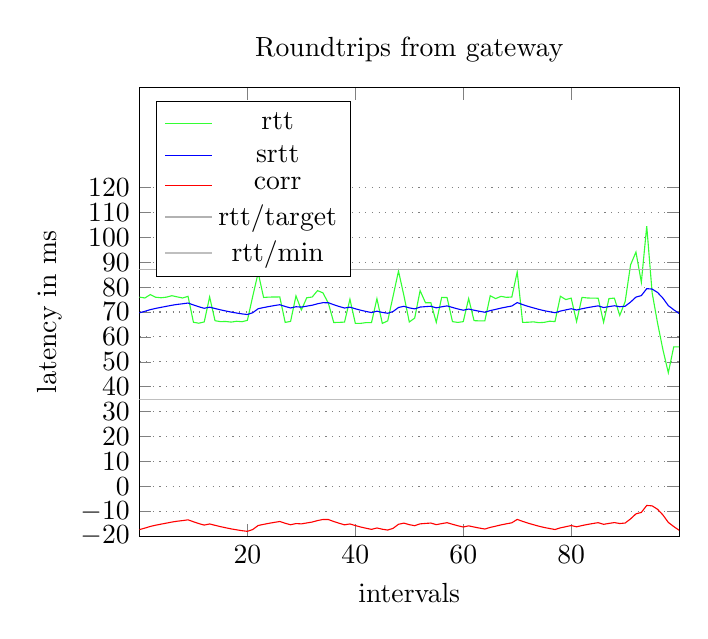
\begin{tikzpicture}\begin{axis}[
title={Roundtrips from gateway},
xlabel={intervals}, ylabel={latency in ms},
xmin=0, xmax=700,ymin=-20, ymax=160,
xtick={100,200,300,400,500,600},
xmin=000, xmax=100,ymin=-20, ymax=160,
xtick={20,40,60,80},
ytick={-40,-30,-20,-10,0,10,20,30,40,50,60,70,80,90,100,110,120},
legend pos=north west, grid style={dotted,gray},ymajorgrids=true,]
\addplot[ color=green!80 ] coordinates {(0,75.991)(1,75.643)(2,76.992)(3,75.942)(4,75.731)(5,75.976)(6,76.558)(7,76.086)(8,75.639)(9,76.307)(10,65.898)(11,65.512)(12,66.03)(13,76.055)(14,66.524)(15,66.15)(16,66.203)(17,65.961)(18,66.293)(19,66.116)(20,66.664)(21,76.432)(22,85.783)(23,75.854)(24,76.0)(25,76.035)(26,76.066)(27,65.843)(28,66.239)(29,76.472)(30,70.825)(31,75.732)(32,76.023)(33,78.602)(34,77.69)(35,73.576)(36,65.8)(37,65.849)(38,65.961)(39,75.15)(40,65.47)(41,65.462)(42,65.755)(43,65.774)(44,75.363)(45,65.433)(46,66.441)(47,76.399)(48,86.451)(49,76.611)(50,66.0)(51,67.571)(52,78.592)(53,73.736)(54,73.725)(55,65.851)(56,75.874)(57,75.814)(58,66.144)(59,65.832)(60,66.148)(61,75.422)(62,66.544)(63,66.444)(64,66.483)(65,76.539)(66,75.392)(67,76.299)(68,75.898)(69,76.036)(70,86.118)(71,65.827)(72,65.901)(73,66.057)(74,65.734)(75,65.848)(76,66.321)(77,66.169)(78,76.336)(79,75.002)(80,75.583)(81,66.182)(82,75.885)(83,75.644)(84,75.573)(85,75.548)(86,65.896)(87,75.396)(88,75.595)(89,68.621)(90,74.196)(91,88.914)(92,94.082)(93,81.974)(94,104.521)(95,77.751)(96,65.6)(97,54.879)(98,45.63)(99,56.024)(100,55.99)};\addlegendentry{rtt}
\addplot[ color=blue ] coordinates {(0,69.6957886491)(1,70.2905097842)(2,70.9606588058)(3,71.4587929252)(4,71.8860136327)(5,72.2950122694)(6,72.7213110425)(7,73.0577799382)(8,73.3159019444)(9,73.61501175)(10,72.843310575)(11,72.1101795175)(12,71.5021615657)(13,71.9574454092)(14,71.4141008682)(15,70.8876907814)(16,70.4192217033)(17,69.9733995329)(18,69.6053595797)(19,69.2564236217)(20,68.9971812595)(21,69.7406631336)(22,71.3448968202)(23,71.7958071382)(24,72.2162264244)(25,72.5981037819)(26,72.9448934037)(27,72.2347040634)(28,71.635133657)(29,72.1188202913)(30,71.9894382622)(31,72.363694436)(32,72.7296249924)(33,73.3168624931)(34,73.7541762438)(35,73.7363586194)(36,72.9427227575)(37,72.2333504817)(38,71.6061154336)(39,71.9605038902)(40,71.3114535012)(41,70.7265081511)(42,70.229357336)(43,69.7838216024)(44,70.3417394421)(45,69.8508654979)(46,69.5098789481)(47,70.1987910533)(48,71.824011948)(49,72.3027107532)(50,71.6724396779)(51,71.2622957101)(52,71.9952661391)(53,72.1693395252)(54,72.3249055726)(55,71.6775150154)(56,72.0971635138)(57,72.4688471625)(58,71.8363624462)(59,71.2359262016)(60,70.7271335814)(61,71.1966202233)(62,70.731358201)(63,70.3026223809)(64,69.9206601428)(65,70.5824941285)(66,71.0634447157)(67,71.5870002441)(68,72.0181002197)(69,72.4198901977)(70,73.7897011779)(71,72.9934310601)(72,72.2841879541)(73,71.6614691587)(74,71.0687222428)(75,70.5466500186)(76,70.1240850167)(77,69.728576515)(78,70.3893188635)(79,70.8505869772)(80,71.3238282795)(81,70.8096454515)(82,71.3171809064)(83,71.7498628157)(84,72.1321765342)(85,72.4737588807)(86,71.8159829927)(87,72.1739846934)(88,72.5160862241)(89,72.1265776017)(90,72.3335198415)(91,73.9915678573)(92,76.0006110716)(93,76.5979499644)(94,79.390254968)(95,79.2263294712)(96,77.8636965241)(97,75.5652268717)(98,72.5717041845)(99,70.9169337661)(100,69.4242403894)};\addlegendentry{srtt}
\addplot[ color=red ] coordinates {(0,-17.3492113509)(1,-16.7544902158)(2,-16.0843411942)(3,-15.5862070748)(4,-15.1589863673)(5,-14.7499877306)(6,-14.3236889575)(7,-13.9872200618)(8,-13.7290980556)(9,-13.42998825)(10,-14.201689425)(11,-14.9348204825)(12,-15.5428384343)(13,-15.0875545908)(14,-15.6308991318)(15,-16.1573092186)(16,-16.6257782967)(17,-17.0716004671)(18,-17.4396404203)(19,-17.7885763783)(20,-18.0478187405)(21,-17.3043368664)(22,-15.7001031798)(23,-15.2491928618)(24,-14.8287735756)(25,-14.4468962181)(26,-14.1001065963)(27,-14.8102959366)(28,-15.409866343)(29,-14.9261797087)(30,-15.0555617378)(31,-14.681305564)(32,-14.3153750076)(33,-13.7281375069)(34,-13.2908237562)(35,-13.3086413806)(36,-14.1022772425)(37,-14.8116495183)(38,-15.4388845664)(39,-15.0844961098)(40,-15.7335464988)(41,-16.3184918489)(42,-16.815642664)(43,-17.2611783976)(44,-16.7032605579)(45,-17.1941345021)(46,-17.5351210519)(47,-16.8462089467)(48,-15.220988052)(49,-14.7422892468)(50,-15.3725603221)(51,-15.7827042899)(52,-15.0497338609)(53,-14.8756604748)(54,-14.7200944274)(55,-15.3674849846)(56,-14.9478364862)(57,-14.5761528375)(58,-15.2086375538)(59,-15.8090737984)(60,-16.3178664186)(61,-15.8483797767)(62,-16.313641799)(63,-16.7423776191)(64,-17.1243398572)(65,-16.4625058715)(66,-15.9815552843)(67,-15.4579997559)(68,-15.0268997803)(69,-14.6251098023)(70,-13.2552988221)(71,-14.0515689399)(72,-14.7608120459)(73,-15.3835308413)(74,-15.9762777572)(75,-16.4983499814)(76,-16.9209149833)(77,-17.316423485)(78,-16.6556811365)(79,-16.1944130228)(80,-15.7211717205)(81,-16.2353545485)(82,-15.7278190936)(83,-15.2951371843)(84,-14.9128234658)(85,-14.5712411193)(86,-15.2290170073)(87,-14.8710153066)(88,-14.5289137759)(89,-14.9184223983)(90,-14.7114801585)(91,-13.0534321427)(92,-11.0443889284)(93,-10.4470500356)(94,-7.654745032)(95,-7.8186705288)(96,-9.18130347592)(97,-11.4797731283)(98,-14.4732958155)(99,-16.1280662339)(100,-17.6207596106)};\addlegendentry{corr}
\addplot[ color=gray!60 ] coordinates {(0,87.045)(1,87.045)(2,87.045)(3,87.045)(4,87.045)(5,87.045)(6,87.045)(7,87.045)(8,87.045)(9,87.045)(10,87.045)(11,87.045)(12,87.045)(13,87.045)(14,87.045)(15,87.045)(16,87.045)(17,87.045)(18,87.045)(19,87.045)(20,87.045)(21,87.045)(22,87.045)(23,87.045)(24,87.045)(25,87.045)(26,87.045)(27,87.045)(28,87.045)(29,87.045)(30,87.045)(31,87.045)(32,87.045)(33,87.045)(34,87.045)(35,87.045)(36,87.045)(37,87.045)(38,87.045)(39,87.045)(40,87.045)(41,87.045)(42,87.045)(43,87.045)(44,87.045)(45,87.045)(46,87.045)(47,87.045)(48,87.045)(49,87.045)(50,87.045)(51,87.045)(52,87.045)(53,87.045)(54,87.045)(55,87.045)(56,87.045)(57,87.045)(58,87.045)(59,87.045)(60,87.045)(61,87.045)(62,87.045)(63,87.045)(64,87.045)(65,87.045)(66,87.045)(67,87.045)(68,87.045)(69,87.045)(70,87.045)(71,87.045)(72,87.045)(73,87.045)(74,87.045)(75,87.045)(76,87.045)(77,87.045)(78,87.045)(79,87.045)(80,87.045)(81,87.045)(82,87.045)(83,87.045)(84,87.045)(85,87.045)(86,87.045)(87,87.045)(88,87.045)(89,87.045)(90,87.045)(91,87.045)(92,87.045)(93,87.045)(94,87.045)(95,87.045)(96,87.045)(97,87.045)(98,87.045)(99,87.045)(100,87.045)};\addlegendentry{rtt/target}
\addplot[ color=gray!50  ] coordinates {(0,34.818)(1,34.818)(2,34.818)(3,34.818)(4,34.818)(5,34.818)(6,34.818)(7,34.818)(8,34.818)(9,34.818)(10,34.818)(11,34.818)(12,34.818)(13,34.818)(14,34.818)(15,34.818)(16,34.818)(17,34.818)(18,34.818)(19,34.818)(20,34.818)(21,34.818)(22,34.818)(23,34.818)(24,34.818)(25,34.818)(26,34.818)(27,34.818)(28,34.818)(29,34.818)(30,34.818)(31,34.818)(32,34.818)(33,34.818)(34,34.818)(35,34.818)(36,34.818)(37,34.818)(38,34.818)(39,34.818)(40,34.818)(41,34.818)(42,34.818)(43,34.818)(44,34.818)(45,34.818)(46,34.818)(47,34.818)(48,34.818)(49,34.818)(50,34.818)(51,34.818)(52,34.818)(53,34.818)(54,34.818)(55,34.818)(56,34.818)(57,34.818)(58,34.818)(59,34.818)(60,34.818)(61,34.818)(62,34.818)(63,34.818)(64,34.818)(65,34.818)(66,34.818)(67,34.818)(68,34.818)(69,34.818)(70,34.818)(71,34.818)(72,34.818)(73,34.818)(74,34.818)(75,34.818)(76,34.818)(77,34.818)(78,34.818)(79,34.818)(80,34.818)(81,34.818)(82,34.818)(83,34.818)(84,34.818)(85,34.818)(86,34.818)(87,34.818)(88,34.818)(89,34.818)(90,34.818)(91,34.818)(92,34.818)(93,34.818)(94,34.818)(95,34.818)(96,34.818)(97,34.818)(98,34.818)(99,34.818)(100,34.818)};\addlegendentry{rtt/min}
\end{axis}\end{tikzpicture}
\caption{gw/test/alpha/0.1/rtttarget/2.5/diff/0.98/slope/0.15/zommed}
\label{fig:gw/test/alpha/0.1/rtttarget/2.5/diff/0.98/slope/0.15/zommed}
\end{figure}



\begin{figure}\centering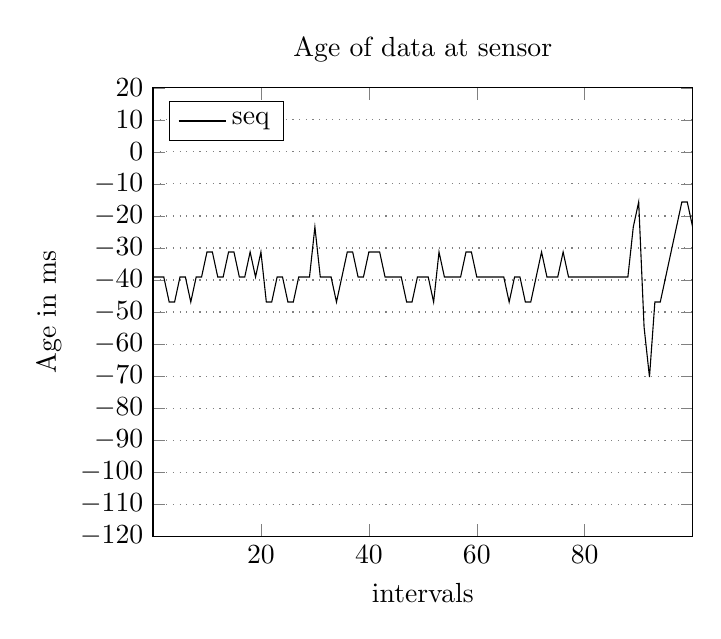
\begin{tikzpicture}\begin{axis}[
title={Age of data at sensor},
xlabel={intervals}, ylabel={Age in ms},
xmin=000, xmax=100,ymin=-120, ymax=20,
xtick={20,40,60,80},
ytick={-120,-110, -100,-90,-80,-70,-60,-50,-40,-30,-20,-10,0,10,20},
legend pos=north west, grid style={dotted,gray},ymajorgrids=true,]
\addplot[  ] coordinates {(0,-39.0625)(1,-39.0625)(2,-39.0625)(3,-46.875)(4,-46.875)(5,-39.0625)(6,-39.0625)(7,-46.875)(8,-39.0625)(9,-39.0625)(10,-31.25)(11,-31.25)(12,-39.0625)(13,-39.0625)(14,-31.25)(15,-31.25)(16,-39.0625)(17,-39.0625)(18,-31.25)(19,-39.0625)(20,-31.25)(21,-46.875)(22,-46.875)(23,-39.0625)(24,-39.0625)(25,-46.875)(26,-46.875)(27,-39.0625)(28,-39.0625)(29,-39.0625)(30,-23.4375)(31,-39.0625)(32,-39.0625)(33,-39.0625)(34,-46.875)(35,-39.0625)(36,-31.25)(37,-31.25)(38,-39.0625)(39,-39.0625)(40,-31.25)(41,-31.25)(42,-31.25)(43,-39.0625)(44,-39.0625)(45,-39.0625)(46,-39.0625)(47,-46.875)(48,-46.875)(49,-39.0625)(50,-39.0625)(51,-39.0625)(52,-46.875)(53,-31.25)(54,-39.0625)(55,-39.0625)(56,-39.0625)(57,-39.0625)(58,-31.25)(59,-31.25)(60,-39.0625)(61,-39.0625)(62,-39.0625)(63,-39.0625)(64,-39.0625)(65,-39.0625)(66,-46.875)(67,-39.0625)(68,-39.0625)(69,-46.875)(70,-46.875)(71,-39.0625)(72,-31.25)(73,-39.0625)(74,-39.0625)(75,-39.0625)(76,-31.25)(77,-39.0625)(78,-39.0625)(79,-39.0625)(80,-39.0625)(81,-39.0625)(82,-39.0625)(83,-39.0625)(84,-39.0625)(85,-39.0625)(86,-39.0625)(87,-39.0625)(88,-39.0625)(89,-23.4375)(90,-15.625)(91,-54.6875)(92,-70.3125)(93,-46.875)(94,-46.875)(95,-39.0625)(96,-31.25)(97,-23.4375)(98,-15.625)(99,-15.625)(100,-23.4375)};\addlegendentry{seq}
\end{axis}\end{tikzpicture}
\caption{sensor/test/alpha/0.1/rtttarget/2.5/diff/0.98/slope/0.15/zommed}
\label{fig:sensor/test/alpha/0.1/rtttarget/2.5/diff/0.98/slope/0.15/zommed}
\end{figure}


